% #######################################
% ########### FILL THESE IN #############
% #######################################
\def\mytitle{Coursework Report}
\def\mykeywords{Edinburgh Napier University, Web Technologies}
\def\myauthor{Samuel Cattanach}
\def\contact{40276600@napier.ac.uk}
\def\mymodule{Web Technologies (SET08101)}
% #######################################
% #### YOU DON'T NEED TO TOUCH BELOW ####
% #######################################
\documentclass[10pt, a4paper]{article}
\usepackage[a4paper,outer=1.5cm,inner=1.5cm,top=1.75cm,bottom=1.5cm]{geometry}
\twocolumn
\usepackage{graphicx}
\graphicspath{{./images/}}
%colour our links, remove weird boxes
\usepackage[colorlinks,linkcolor={black},citecolor={blue!80!black},urlcolor={blue!80!black}]{hyperref}
%Stop indentation on new paragraphs
\usepackage[parfill]{parskip}
%% Arial-like font
\IfFileExists{uarial.sty}
{
    \usepackage[english]{babel}
    \usepackage[T1]{fontenc}
    \usepackage{uarial}
    \renewcommand{\familydefault}{\sfdefault}
}{
    \GenericError{}{Couldn't find Arial font}{ you may need to install 'nonfree' fonts on your system}{}
    \usepackage{lmodern}
    \renewcommand*\familydefault{\sfdefault}
}
%Napier logo top right
\usepackage{watermark}
%Lorem Ipusm dolor please don't leave any in you final report ;)
\usepackage{lipsum}
\usepackage{xcolor}
\usepackage{listings}
%give us the Capital H that we all know and love
\usepackage{float}
%tone down the line spacing after section titles
\usepackage{titlesec}
%Cool maths printing
\usepackage{amsmath}
%PseudoCode
\usepackage{algorithm2e}

\titlespacing{\subsection}{0pt}{\parskip}{-3pt}
\titlespacing{\subsubsection}{0pt}{\parskip}{-\parskip}
\titlespacing{\paragraph}{0pt}{\parskip}{\parskip}
\newcommand{\figuremacro}[5]{
    \begin{figure}[#1]
        \centering
        \includegraphics[width=#5\columnwidth]{#2}
        \caption[#3]{\textbf{#3}#4}
        \label{fig:#2}
    \end{figure}
}

\lstset{
	escapeinside={/*@}{@*/}, language=C++,
	basicstyle=\fontsize{8.5}{12}\selectfont,
	numbers=left,numbersep=2pt,xleftmargin=2pt,frame=tb,
    columns=fullflexible,showstringspaces=false,tabsize=4,
    keepspaces=true,showtabs=false,showspaces=false,
    backgroundcolor=\color{white}, morekeywords={inline,public,
    class,private,protected,struct},captionpos=t,lineskip=-0.4em,
	aboveskip=10pt, extendedchars=true, breaklines=true,
	prebreak = \raisebox{0ex}[0ex][0ex]{\ensuremath{\hookleftarrow}},
	keywordstyle=\color[rgb]{0,0,1},
	commentstyle=\color[rgb]{0.133,0.545,0.133},
	stringstyle=\color[rgb]{0.627,0.126,0.941}
}

\thiswatermark{\centering \put(336.5,-38.0){
\includegraphics[scale=0.8]{logo}} }
\title{\mytitle}
\author{\myauthor\hspace{1em}\\\contact\\Edinburgh Napier University\hspace{0.5em}-\hspace{0.5em}\mymodule}
\date{}
\hypersetup{pdfauthor=\myauthor,pdftitle=\mytitle,pdfkeywords=\mykeywords}
\sloppy
% ###################################################################################
% ########### START FROM HERE #######################################################
% ###################################################################################
\begin{document}
    \maketitle
    \textbf{Keywords -- }{\mykeywords}
    
    \section{Introduction}
    This website demonstrates the encryption and decryption of text using several different cyphers implemented using JavaScript. It consists of several pages with different cyphers, information on how they encrypt text, and a page with the typographical and presentational design used consistently throughout the website. JavaScript files have been used for each cypher in order to encrypt and decrypt text input by the user. A CSS file has been used with each page to format the elements correctly. 
\\\\  I chose to implement two types of Caesar cyphers, or simple substitution cyphers, ROT13 and Affine, and Base64 encoding. I chose these cyphers as they effectively demonstrate how basic encoding of text works in different ways. By giving the user the option of using ROT1 to ROT25, they can see clearly how the text is encrypted as the rotation changes. Binary-to-text encoding such as Base64 demonstrates a different type of encryption as text is represented as a byte sequence of 8-bit-padded ASCII characters encoded in MIME's Base64. \cite{Base64}


	\section{Software Design}
	Before developing the html and JavaScript files, I 
	constructed a list of the required elements of the website, as well as sketches of the layout to be later implemented with CSS. A navigation diagram was created, showing the HTML pages relation to each other and how the user will navigate to each page.
	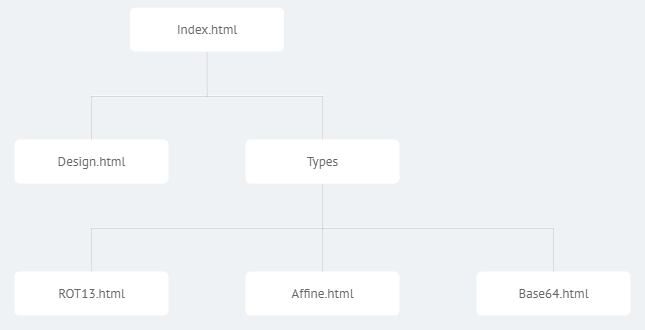
\includegraphics[scale=0.52]{tree} 
	
	
	\section{Implementation}
	%Short description of your site’s implementation including screenshots. 
	Each page in the website can be navigated to by links in the navigation bar. The index page contains a brief description of cyphers and cryptography along with pictures of cyphers. The navigation bar contains a drop-down menu with links to three cypher pages. the menu is implemented using a JavaScript script, allowing it to be made visible when clicked on. The cypher pages contain text areas that allow the user to enter text and displays it in the corresponding text area as encrypted text.
	\\
	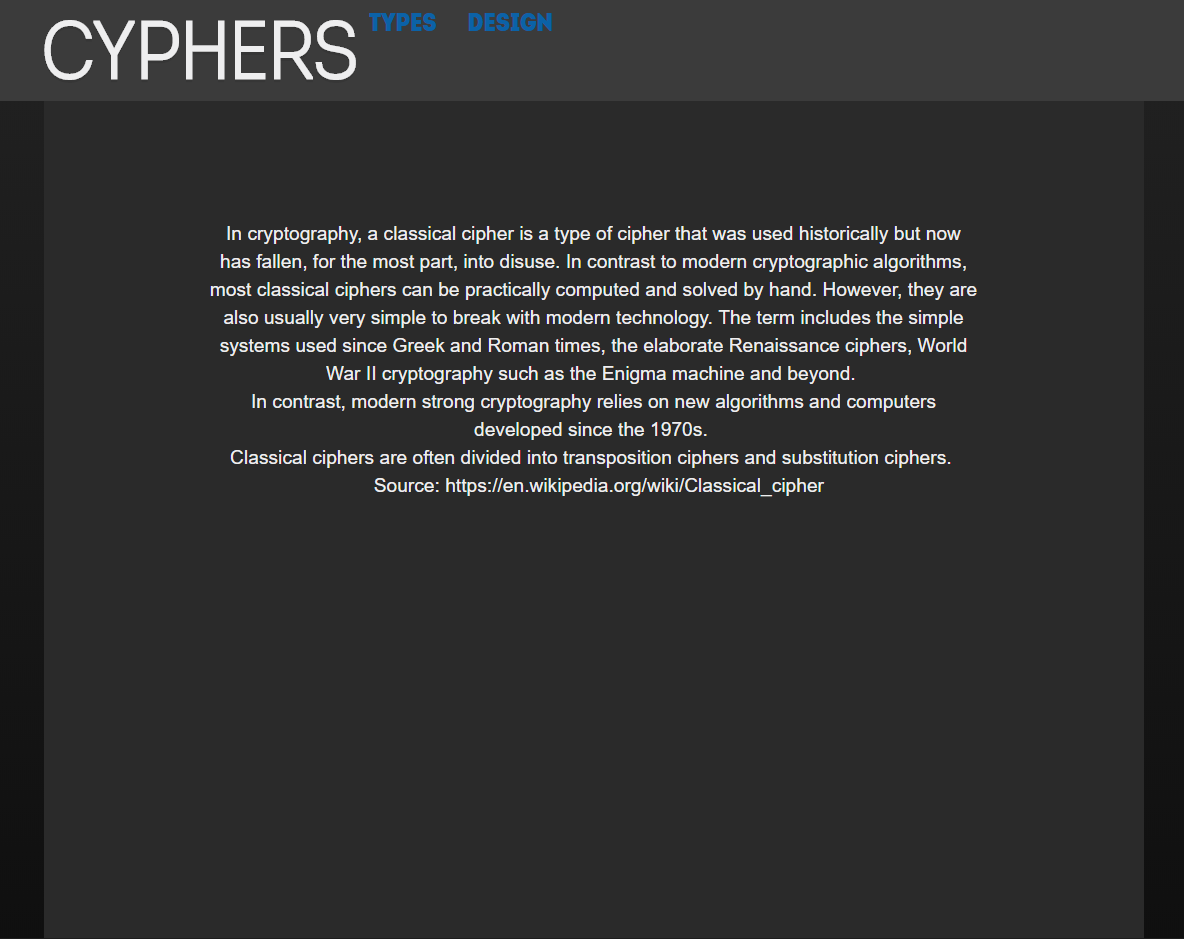
\includegraphics[scale=0.314]{index} 
	Index page
	\\\\
	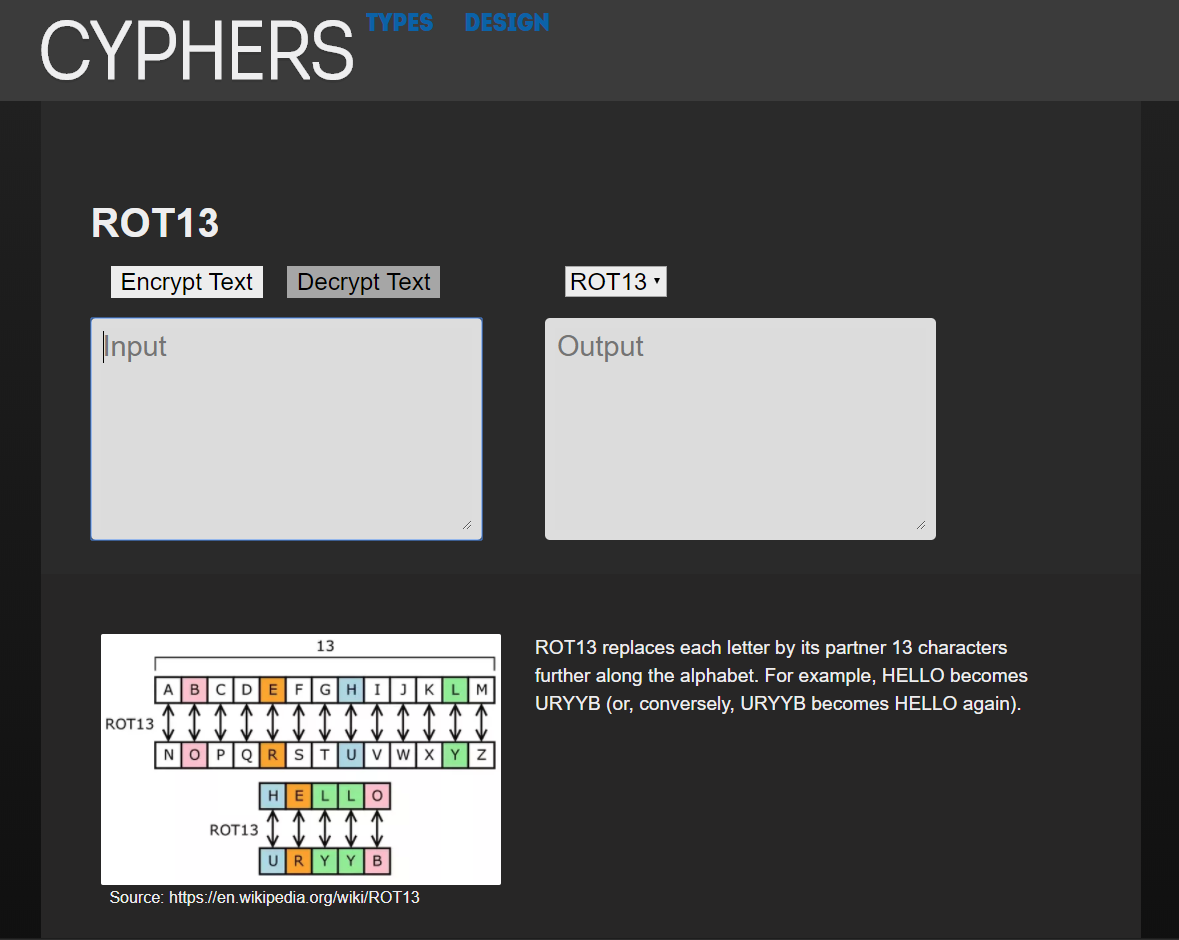
\includegraphics[scale=0.293]{rot13}
	ROT13 page
	\\\\
	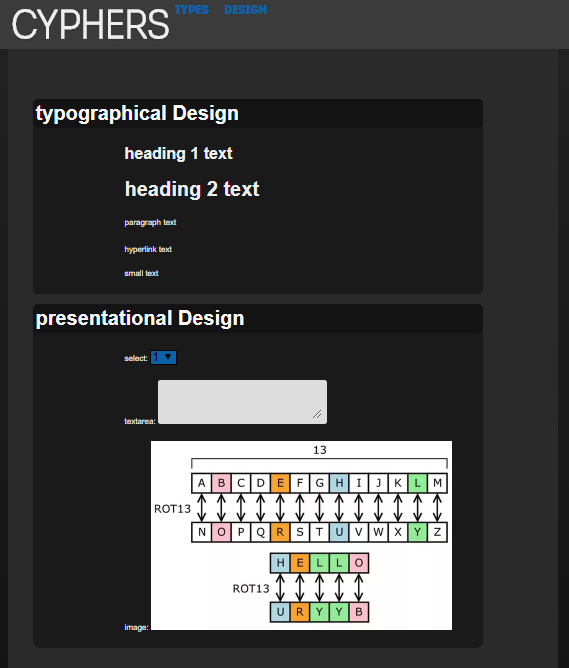
\includegraphics[scale=0.59]{design}
	Design page
	\\\\
	
	\section{Critical Evaluation}
	%Critical evaluation of your implementation. Points to consider discussing in this section are:
    
	\subsection{Requirements Comparison}
	%A comparison against the requirements set out in this document
	    When compared to the original plans, sketches and list of requirements, I believe the finished website meets all of the requirements and elements I initially intended to include. Some elements, such as the colour and layout of certain objects differ from the original plan as my opinion and preference has changed throughout the development process. Recognising certain visual impairments users may have, accessibility and usability was important in the design of the website.

	\subsection{Possible Improvements}
    %• Possible improvements to your application, for example, what did you miss out?
	In my evaluation of the overall website, certain elements stood out in my mind to have the potential to include more features and to be implemented more seamlessly into the design. Several HTML elements varied from the intended outcome, in terms of the positional and style relevant to other elements but still function at intended and do not effect the user experience or accessibility negatively. 
	
	
	\section{Personal Evaluation}
	%reflecting on what you learned, the challenges you faced, the methods you used to overcome challenges, and you feel you performed. 
	Throughout the planning and development stage of this website, my understanding and overall knowledge of markup languages like HTML and CSS, and JavaScript has expanded from the experiences I have gained throughout this process. My knowledge of the subject has been aided by several sources of information, from different tutorials and documentation available on the internet and from material available on the SET08101 module. Many challenges that occurred along the development stage, were resolved through the use of official documentation of . One example of a problem I faced was in my attempt to implement a dynamic drop-down menu that would be made visible when clicked on by the user. To resolve the issues I faced with this element I referenced material from the web technologies workbook as well as tutorials provided by w3schools that provide information on how to allow the menu to be interacted with. \\cite{w3schools}
	
	
    
    %You must provide a reference for every resource used that you have not created yourself – for example, additional image, sound, video, or software library resources
	\bibliographystyle{ieeetr}
	
	\bibliography{references}	

		
\end{document}
